\subsection{Konsepter}
For å finne ulike konsepter og ideer for brukergrensesnittet ble det gjennomført en brainstorm.
Noen av ideene fra denne brainstormen er oppsummert her.

\paragraph{Tid og splittid}
Konseptet bestod av en tabell med rundetider og splittider.
Splittidene listes opp horisontalt for hver runde, og rundene listes opp vertikalt.
Tidene skal kunne vises enten som brukt tid, eller differansen mellom planlagt og brukt tid.
Dette gjør det lett å sammenligne de ulike rundene, og planlegge ulike hastigheter for disse.

\paragraph{Trending av måledata}
Siden måledata hele tiden endrer seg, vil det være interessant å se hvordan dataene har endret seg over tid.

\paragraph{Bruk av farger}
Å benytte farger til måledata vil kunne gjøre det enklere for en bruker å vite betydningen av en måleverdi.

\paragraph{Skjuling av måleverdier}
Siden måledata er mest interessante når de ikke er innen normale verdier, kan disse skjules når de normale.
Dette vil gi brukeren mindre data å holde orden på.

\subsection{Vurdering}
For å vurdere disse konseptene ble ecomarathon-teamet benyttet.
Årsaken til dette var at gruppa ikke hadde klare nok rammer til å gjøre en vurdering på egen hånd.
Tegningen til Hans (Figur \ref{gui-concept}) ble benyttet som et utgangspunkt under denne vurderingen.
Det ble klart at tid var langt mer viktig enn fart, så hovedskjermbildet ble det avgjort skulle først og fremst inneholde rundetider og et kart over banen. 
Trending av data ble det klart burde kombineres med å holde disse skjult når disse ikke var interessante.
Ideen om å vise splittider og anbefalt hastighet ble etter hvert avvist siden dette ville være vanskelig å implementere på en tilfredsstillende måte.
Et av problemene er at man ikke har nøyaktige avstander på banen, men også at man er nødt til å stoppe en gang for hver runde.

\begin{figure}[H]
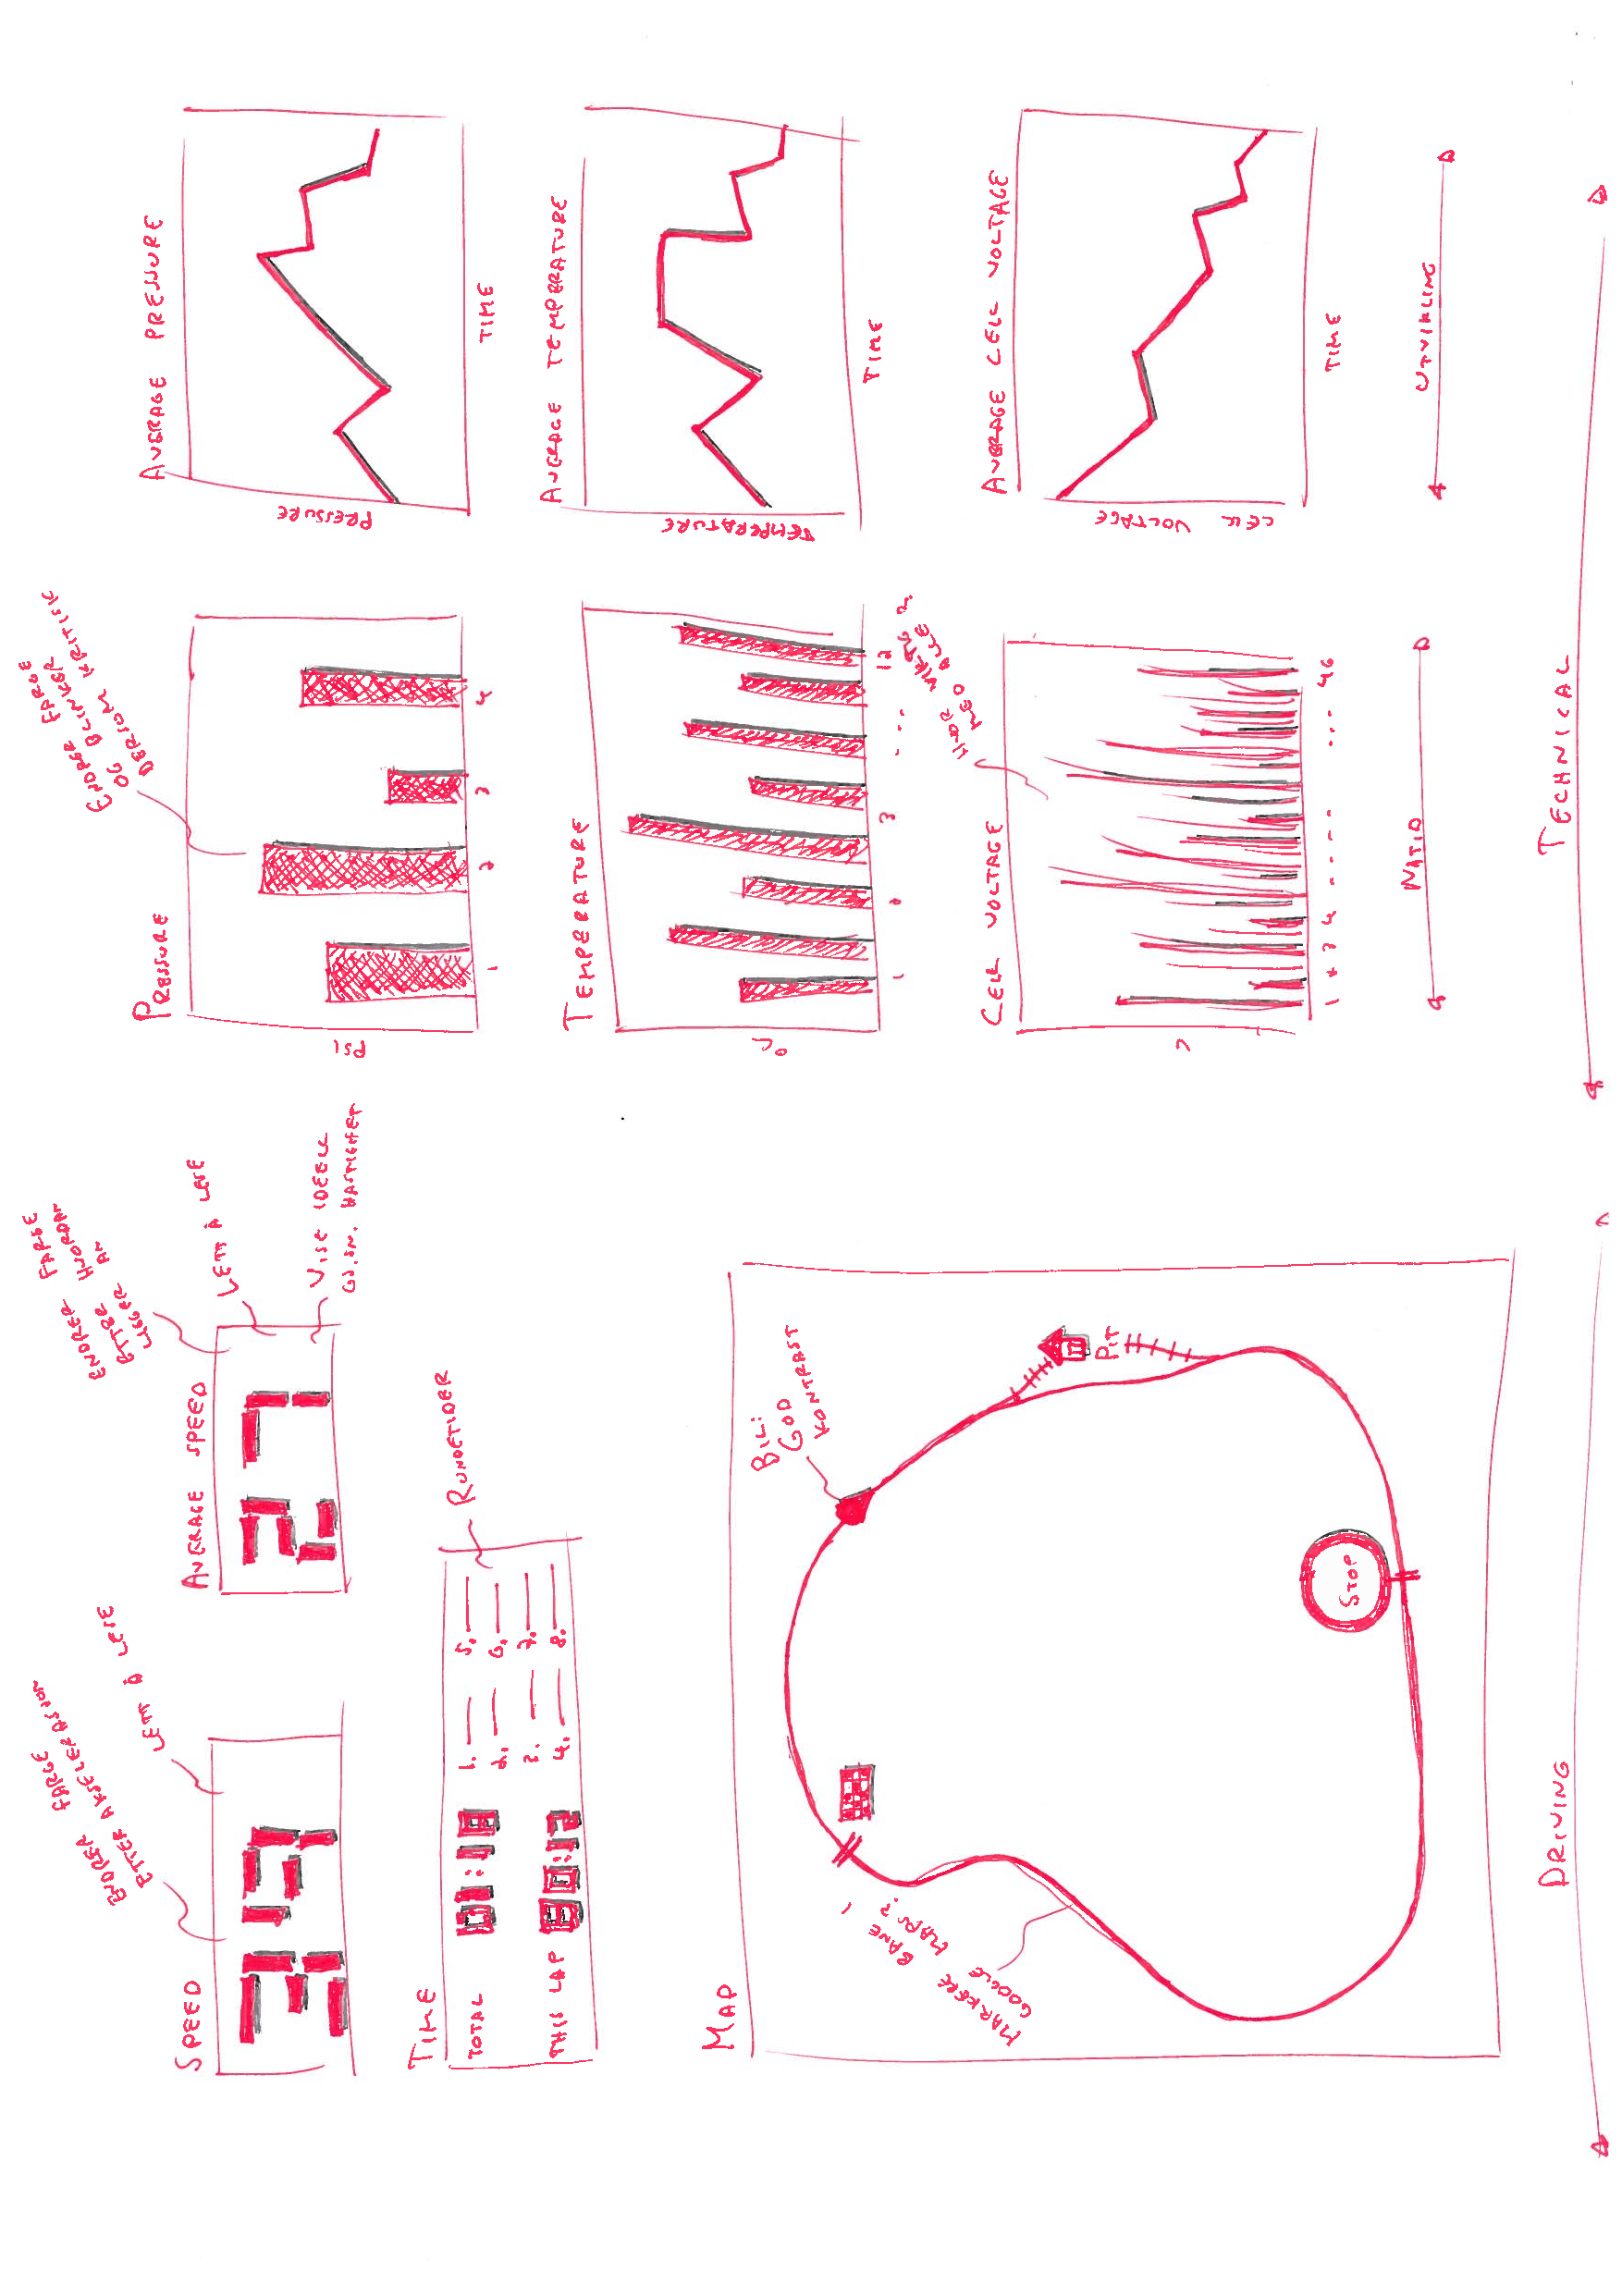
\includegraphics[width=\textwidth]{images/gui_concept_hans.pdf}
\caption{GUI-konsept} 
\label{gui-concept}
\end{figure}
